
分布式系统(如云本机架构)带来了一些独特的挑战。在给定时间工作的不同服务的数量之多,使得研究组件的性能十分不便。

在单系统中,日志记录和性能监控通常就足够了。对于分布式系统,甚至日志记录也需要一个设计选择。不同的组件产生不同的日志格式。那些日志总得有个地方存放。将它们与交付它们的服务结合在一起,将很难在宕机情况下了解全局状态。此外,由于微服务的生命周期可能很短,可能希望将日志的生命周期与提供日志的服务或承载该服务的机器的生命周期分离开来。

在第13章中,描述了统一的日志记录层如何帮助管理日志。但是日志只显示系统中给定点发生的事情。要从单个事务的角度查看问题,需要使用不同的方法。

这时就需要进行跟踪了。

\subsubsubsection{15.3.1\hspace{0.2cm}跟踪与日志记录有何不同}

跟踪是一种特殊形式的日志记录,提供的信息级别比日志低。包括所有函数调用、参数、大小和执行时间。还包含正在处理的事务的ID。通过这些细节,可以重新组合,并查看给定事务通过系统时的生命周期。

跟踪中显示的性能信息,可以发现系统中的瓶颈和次优组件。

日志通常由操作人员和开发人员读取,所以它们是人类可读的,对跟踪没有这样的要求。要查看轨迹,需要使用专用的可视化程序。这意味着即使跟踪更详细,也可能比日志占用更少的空间。

下面的图表是单个跟踪的概述:

\begin{center}
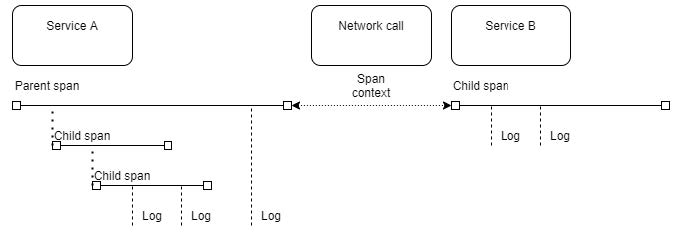
\includegraphics[width=0.9\textwidth]{content/4/chapter15/images/1.jpg}\\
图15.1 -单个跟踪
\end{center}

两个服务在一个网络上通信。在服务A中,有一个父跨度,它包含一个子跨度和一个日志。子跨度通常对应于更深层的函数调用,日志表示最小的一条信息。每一个都是计时的,并且可能包含额外的信息。

对服务B的网络调用保存了时间的上下文。即使服务B是在另一台机器上的不同进程中执行的,因为事务ID保留,所有信息都可以在稍后重新加载。

从重新加载跟踪中获得的一个额外信息是,分布式系统中服务之间的依赖关系图。由于跟踪包含整个调用链,因此可以将此信息可视化并检查意外依赖项。

\subsubsubsection{15.2.2\hspace{0.2cm}选择跟踪解决方案}

实现跟踪时,有几种可能的解决方案可供选择,可以使用自托管和托管工具来测试应用程序。我们将简要介绍托管类,并重点介绍自托管类。

\hspace*{\fill} \\ %插入空行
\noindent
\textbf{Jaeger和OpenTracing}

分布式跟踪的标准之一是Jaeger的作者提出的OpenTracing。Jaeger是为云本地应用程序构建的跟踪程序,解决了监视分布式事务和传播跟踪上下文的问题。它的用途如下:

\begin{itemize}
\item 
性能或延迟优化

\item 
执行原因分析

\item 
分析服务间的依赖关系
\end{itemize}

OpenTracing是一个开放标准,提供了一个独立于所使用的跟踪程序的API。这意味着当应用程序使用OpenTracing测试时,可以避免锁定在一个特定的供应商。如果在某些时候,可以从Jaeger切换到Zipkin、DataDog或任何其他兼容的跟踪程序,从而不必修改整个检测代码。

有许多与OpenTracing兼容的客户端库。还可以找到许多资源,包括解释如何根据需要实现API的教程和文章。OpenTracing官方支持以下语言:

\begin{itemize}
\item 
Go

\item 
JavaScript

\item 
Java

\item 
Python

\item 
Ruby

\item 
PHP

\item 
Objective-C

\item 
C++

\item 
C\#
\end{itemize}

还有一些非官方的库可用,特定的应用程序也可以导出OpenTracing数据。这包括Nginx和Envoy,这两种流行的Web代理。

Jaeger也接受Zipkin格式的样本,将在下一节介绍Zipkin。如果(或依赖项)已经使用Zipkin,则无需将测试从一种格式改写为另一种格式。对于所有新应用程序,建议采用OpenTracing方法。

Jaeger的扩展性也不错。如果想对其进行计算,可以将其作为单个二进制文件或单个应用程序容器运行。可以为生产环境配置Jaeger,使用它自己的后端或支持的外部后端,如Elasticsearch,Cassandra或Kafka。

Jaeger是一个CNCF的毕业项目,已经达到了与Kubernetes、Prometheus或Fluentd相似的成熟水平。正因为如此,我们希望它在其他CNCF应用中得到更多的支持。

\hspace*{\fill} \\ %插入空行
\noindent
\textbf{Zipkin}

Jaeger的主要竞争对手是Zipkin。这是一个较老的项目,这也意味着它更成熟。通常,更高级的项目也会得到更好的支持,但CNCF的支持对Jaeger有利。

Zipkin使用其专有协议来处理跟踪,提供了OpenTracing支持,但是它的成熟度和支持级别可能比不上原生的Jaeger协议。正如前面提到的,还可以配置Jaeger以Zipkin格式收集跟踪。说明这两者至少在某种程度上是可以互换的。

该项目由Apache基金会托管,但不认定为CNCF项目。在开发云原生应用程序时,Jaeger是一个更好的选择。如果正在寻找一种通用的跟踪解决方案,Zipkin也是值得尝试。

Zipkin的一个缺点是没有C++实现。有非官方的库,但它们似乎没有得到很好的支持。使用C++的OpenTracing库是测试C++代码的首选方法。

\subsubsubsection{15.2.3\hspace{0.2cm}使用OpenTracing测试应用程序}

本节将演示如何将Jaeger和OpenTracing插装添加到现有的应用程序中,这里将使用opentrace-cpp和jaeger-client-cpp库。

首先,想要设置跟踪器:

\begin{lstlisting}[style=styleCXX]
#include <jaegertracing/Tracer.h>

void setUpTracer()
{
	// We want to read the sampling server configuration from the
	// environment variables
	auto config = jaegertracing::Config;
	config.fromEnv();
	// Jaeger provides us with ConsoleLogger and NullLogger
	auto tracer = jaegertracing::Tracer::make(
	"customer", config, jaegertracing::logging::consoleLogger());
	opentracing::Tracer::InitGlobal(
	std::static_pointer_cast<opentracing::Tracer>(tracer));
}
\end{lstlisting}

配置采样服务器的两种首选方法是使用环境变量,或者使用YAML配置文件。在使用环境变量时,必须在运行应用程序之前设置它们。需要注意以下几点:

\begin{itemize}
\item 
JAEGER\_AGENT\_HOST: Jaeger代理所在的主机名

\item 
JAEGER\_AGENT\_POR: Jaeger代理正在监听的端口

\item 
JAEGER\_SERVICE\_NAME: 应用程序的名称
\end{itemize}

接下来,配置跟踪程序并提供日志记录实现。如果可用的ConsoleLogger不够用,则可以实现自定义日志记录解决方案。对于具有统一日志记录层的基于容器的应用程序,ConsoleLogger应该足够了。

当设置好跟踪程序后,希望将跨度添加到想要检测的函数中。下面的代码就是这样做的:

\begin{lstlisting}[style=styleCXX]
auto responder::respond(const http_request &request, status_code status,
const json::value &response) -> void {
	auto span = opentracing::Tracer::Global()->StartSpan("respond");
	// ...
}
\end{lstlisting}

稍后可以使用此跨度在给定函数中创建子跨度,也可以作为参数传播到更深层的函数调用:

\begin{lstlisting}[style=styleCXX]
auto responder::prepare_response(const std::string &name, const
std::unique_ptr<opentracing::Span>& parentSpan)
-> std::pair<status_code, json::value> {
	auto span = opentracing::Tracer::Global()->StartSpan(
	"prepare_response", { opentracing::ChildOf(&parentSpan->context())
	});
	return {status_codes::OK,
		json::value::string(string_t("Hello, ") + name + "!")};
}

auto responder::respond(const http_request &request, status_code status)
-> void {
	auto span = opentracing::Tracer::Global()->StartSpan("respond");
	// ...
	auto response = this->prepare_response("Dominic", span);
	// ...
}
\end{lstlisting}

当调用\texttt{opentracing::ChildOf}函数时,就会发生上下文传播。还可以使用\texttt{inject()}和\texttt{extract()}调用通过网络调用传递上下文。













